\documentclass[a4paper,11pt]{article}

%A Few Useful Packages
\usepackage{marvosym}
\usepackage{fontspec} 					%for loading fonts
\usepackage{xunicode,xltxtra,url,parskip} 	%other packages for formatting
\RequirePackage{color,graphicx}
\usepackage[usenames,dvipsnames]{xcolor}
\usepackage[big]{layaureo} 				%better formatting of the A4 page
% an alternative to Layaureo can be ** \usepackage{fullpage} **
\usepackage{supertabular} 				%for Grades
\usepackage{titlesec}					%custom \section
\usepackage{xeCJK}						%chinese
\usepackage{graphicx}
\usepackage{geometry}
\usepackage{wrapfig}

%\geometry{papersize={20cm,15cm}}
\geometry{top=1cm,bottom=1cm}


%Setup hyperref package, and colours for links
\usepackage{hyperref}
\definecolor{linkcolour}{rgb}{0,0.2,0.6}
\hypersetup{colorlinks,breaklinks,urlcolor=linkcolour, linkcolor=linkcolour}

%FONTS
\defaultfontfeatures{Mapping=tex-text}
%\setmainfont[SmallCapsFont = Fontin SmallCaps]{Fontin}
%%% modified for Karol Kozioł for ShareLaTeX use
\setmainfont[
SmallCapsFont = Fontin-SmallCaps.otf,
BoldFont = Fontin-Bold.otf,
ItalicFont = Fontin-Italic.otf
]
{Fontin.otf}
\setCJKmainfont[BoldFont={黑体}]{STXihei} %设置 CJK 主字体为 SimSun (宋体)

%%%

%CV Sections inspired by: 
%http://stefano.italians.nl/archives/26
\titleformat{\section}{\Large\scshape\raggedright}{}{0em}{}[\titlerule]
\titlespacing{\section}{0pt}{3pt}{3pt}
%Tweak a bit the top margin
%\addtolength{\voffset}{-1.3cm}

%Italian hyphenation for the word: ''corporations''
\hyphenation{im-pre-se}

%-------------WATERMARK TEST [**not part of a CV**]---------------
\usepackage[absolute]{textpos}

\setlength{\TPHorizModule}{30mm}
\setlength{\TPVertModule}{\TPHorizModule}
\textblockorigin{2mm}{0.65\paperheight}
\setlength{\parindent}{0pt}

%--------------------BEGIN DOCUMENT----------------------
\begin{document}

%WATERMARK TEST [**not part of a CV**]---------------
%\font\wm=''Baskerville:color=787878'' at 8pt
%\font\wmweb=''Baskerville:color=FF1493'' at 8pt
%{\wm 
%	\begin{textblock}{1}(0,0)
%		\rotatebox{-90}{\parbox{500mm}{
%			Typeset by Alessandro Plasmati with \XeTeX\  \today\ for 
%			{\wmweb \href{http://www.aleplasmati.comuv.com}{aleplasmati.comuv.com}}
%		}
%	}
%	\end{textblock}
%}

\pagestyle{empty} % non-numbered pages

\font\fb=''[cmr10]'' %for use with \LaTeX command

%--------------------TITLE-------------
\par{
		\begin{center}{\Huge 张 \textsc{政}
	}\end{center}
\par}

%--------------------SECTIONS-----------------------------------
%Section: Personal Data
\begin{wrapfigure}{r}{0.19\textwidth} %this figure will be at the right
    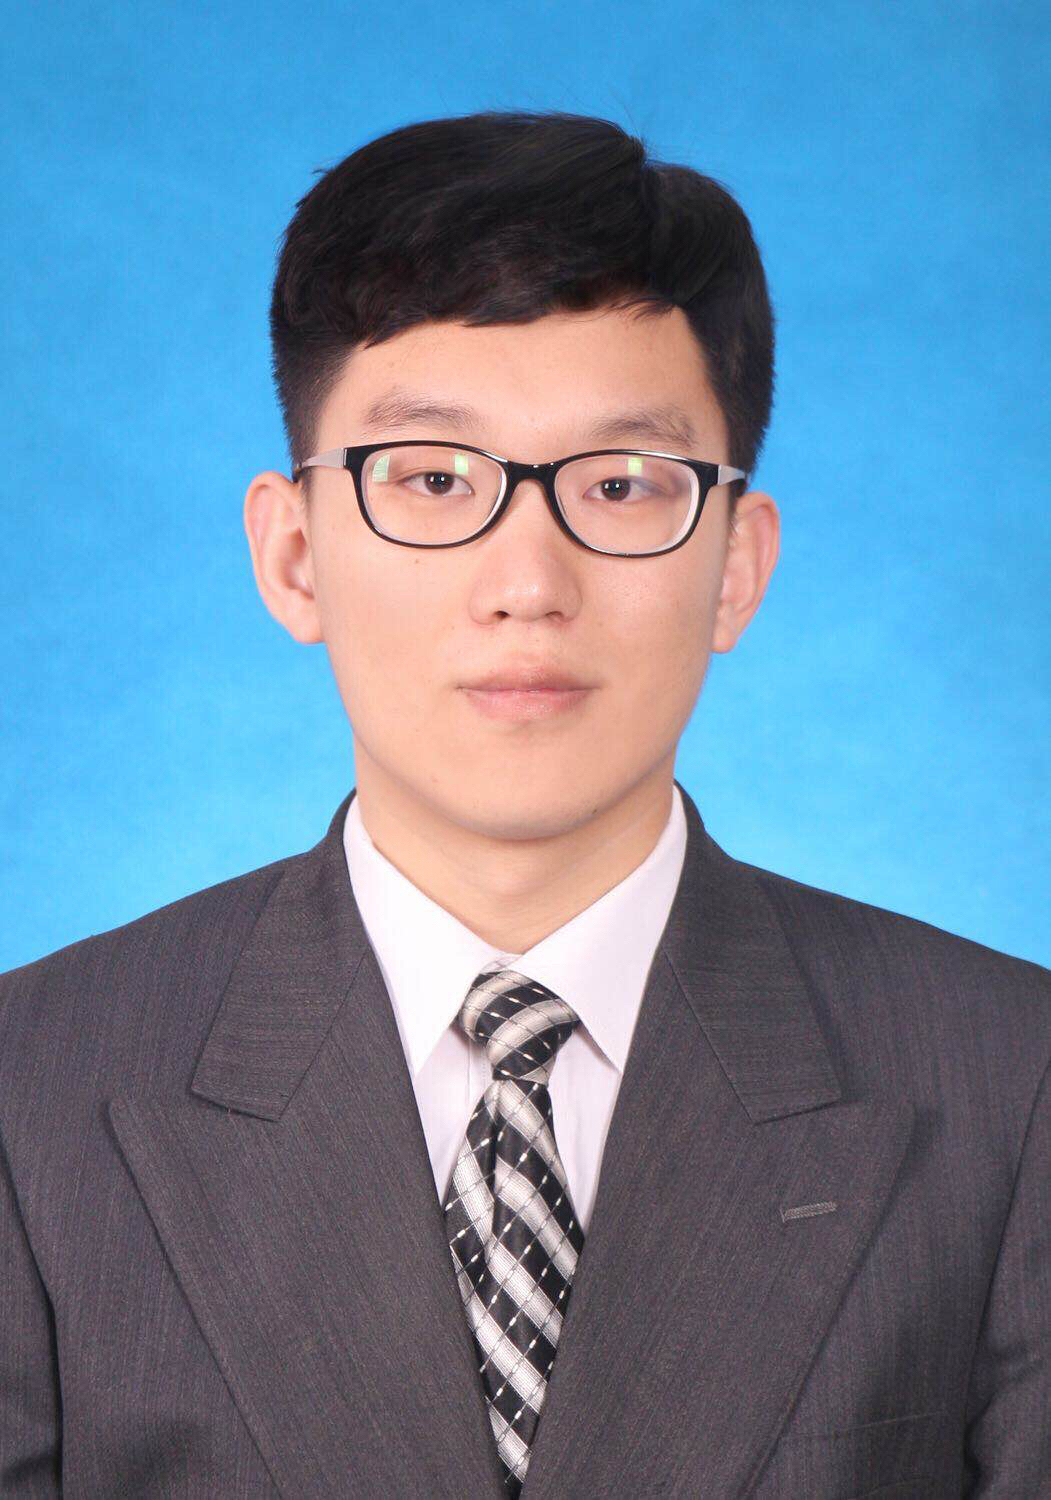
\includegraphics[width=0.19\textwidth]{pic.jpg}
\end{wrapfigure}
\section{基本信息}
\begin{tabular}{rl}
  \textsc{生日:} & 1993.12.03 \\
  \textsc{籍贯:} & 河南省鹤壁市 \\
  \textsc{地址:}   &  上海市闵行区东川路800号上海交通大学\\
  \textsc{手机:}     & 18818272991\\
  \textsc{邮箱:}     & \href{mailto:18818272991@163.com}{18818272991@163.com}\\
  \textsc{博客:}     & \href{https://zzsean.github.io}{https://zzsean.github.io}\\
\end{tabular}



%Section: Education
\section{学习经历}
\begin{tabular}{rl}
\textsc{2012.9} & \bf{本科, 上海交通大学, 电子信息与电气工程学院, 测控技术与仪器专业}\\
& 以专业第一的成绩得到研究生保送资格\\
& 主修课程: 模拟电路, 数字电路, 数据结构, c语言程序设计, python程序设计\\&\\
\textsc{2016.9} & \bf{硕士, 上海交通大学, 电子信息与电气工程学院, 测控技术与仪器专业}\\
& 主修课程: 高级数字信号处理, 微弱信号检测, 视觉检测\\&\\
\textsc{2017.10} & \bf{Coursera Machine Learning课程}\\
& 学习并掌握了传统机器学习的相关原理和算法,如决策树, KNN, LR, SVM\\
& 等, 熟知其推导过程及相应的代码实现\\&\\
\textsc{2017.11} & \bf{Coursera Deep Learning课程 \& 斯坦福大学公开课 CS231n课程}\\
& 了解深度学习的概念,学习常见的深度神经网络模型和序列模型\\
& 熟知其结构特点及相应的代码实现, 并能独立完成一些计算机视觉项目\\
& 学习使用Tensorflow,PyTorch及Keras等开源框架, 学习训练中调参和\\
& 优化的思路和方法\\
\end{tabular}

%Section: Work Experience at the top
\section{实习经历}
\begin{tabular}{r|p{11cm}}
 \textsc{2018.6 - 9} & 华为上海研究所, 海思笛卡尔开发部GPU架构组, 算法工程师 \\&\footnotesize{对已有模型进行测试实验并分析结果, 结合GPU内的相关算法与计算机体系结构等相关知识, 提出项目中相关函数的优化方案; 负责编写了实现工作流程自动化的脚本; 实现远程分布式编译; 熟悉并学习了GPU架构的相关知识, 了解主流的GPU架构及其特点; 学习并掌握OpenGL ES的使用.}\\\multicolumn{2}{c}{} \\
\end{tabular}

%Section: Work Experience at the top
\section{竞赛\&开源项目}
\begin{tabular}{r|p{11cm}}
\textsc{2018.6 - 8} & Kaggle: Google AI Open Images - Object Detection Track (top20\%)\\&\footnotesize{对图片进行目标检测识别, 最后提交的结果包含: 每张图片中所有识别出的物体的类别名称, 置信度和框的位置. 样本集来自Google Open Images, 样本量为170万左右, 600个类别, 平均每张图片中有7个物体. 实现方法为: 使用PyTorch实现YOLOv3的基本模型, 对原始网络的输出表达进行修改以适应比赛要求, 训练样本并适当地调整优化参数.}\\\multicolumn{2}{c}{} \\
\textsc{2018.2} & Generative Adversarial Networks(GAN, 生成对抗网络)\\&\footnotesize{GAN可以用来生成质量很高的图片. 根据论文中所描述的原理, 实现GAN的根本就是生成器与判别器之间的博弈.在这个项目中使用了Tensorflow来完成神经网络框架的搭建, 由于MNIST数据集中的图像特征较为简单, 因此尝试使用了仅含全连接层和加入卷积层的不同神经网络结构实现生成器和判别器, 并尝试了不同的激活函数(如Leaky Relu和Relu)以及Batchnorm的使用, 比较不同网络结构的生成图片的质量.}\\\multicolumn{2}{c}{} \\
\end{tabular}

%Section: Work Experience at the top
\section{竞赛\&开源项目}
\begin{tabular}{r|p{11cm}}
\textsc{2017.12} & Image Caption and Description(图像内容获取和描述)\\{- 2018.1}&\footnotesize{该项目数据集来自微软的COCO数据集, 训练的过程分为两步: 编码和译码. 整个神经网络框架使用Tensorflow搭建, 编码的过程是通过CNN(如 VGG-19)对图像进行特征提取并作为序列模型RNN/LSTM的隐藏层输入; 译码的过程是通过序列模型, 使用词嵌入训练生成对图片内容的文字描述.  }\\\multicolumn{2}{c}{} \\
\textsc{2017.11-12} & Style Transfer(图像风格迁移)\\&\footnotesize{该项目使用Tensorflow搭建神经网络. 实现图片风格转换需要计算两个代价函数: 内容代价函数使用原始图片和生成图片经过CNN网络(如VGG-19)后的高层特征提取进行最小二乘计算而得; 风格代价函数与之相似但是使用的是特征提取后的Gram矩阵进行计算. 预训练风格生成网络可以加速图片转换的速度, 便于进行大量图片单一风格的转换. }
\end{tabular}

%Section: Work Experience at the top
\section{科研经历}
\begin{tabular}{r|p{11cm}}
 \emph{目前} & 电子根尖测定仪 \\&\footnotesize{电子根尖测定仪的设计研究和改进为研究生阶段的主要课题, 主要包括电路的设计, 嵌入式程序的编写, 数据的处理等, 主要涉及的是C语言和MATLAB. 以及针对目前电子根测仪在实际应用中出现的问题进行改善. 并创新性地将神经网络应用其中, 通过不断的调参和网络优化, 有效地提高了测量的准确度以及测量系统地鲁棒性.}\\\multicolumn{2}{c}{} \\
 \textsc{2016.1 - 6} & 主动降噪耳机控制系统 \\&\footnotesize{此研究课题通过主动噪声控制, 利用LMS(最小均方算法)自适应算法, 以Labview为基础搭建一个主动降噪耳机系统, 通过MATLAB进行离线数据验证, 成功实现耳机内的主动降噪.}\\\multicolumn{2}{c}{} \\
\end{tabular}

%Section: Scholarships and additional info
\section{获奖经历\&证书}
\begin{tabular}{rl}
 \textsc{2014}  & 上海交通大学优秀奖学金B等\\
& "E + H" 专项奖学金\\
 \textsc{2015} & 上海交通大学优秀奖学金B等\\
 \textsc{2016} & 上海交通大学2016届优秀毕业生\\
&  上海交通大学研究生一等学业奖学金\\

\end{tabular}

%Section: Languages
\section{语言能力}
\begin{tabular}{rl}
英语: CET6 : 535, 可以流利的阅读英文文献并用英语交流\\
\end{tabular}

\section{计算机能力}
\begin{tabular}{rl}
 编程语言:& Python, ~~C\&C++, ~~Java, ~~MySQL \\
 编程工具:& MATLAB, ~~Labview, ~~Tensorflow, ~~OpenGL, ~~{\fb \LaTeX}\setmainfont[SmallCapsFont=Fontin-SmallCaps.otf]{Fontin.otf}\\
 操作系统:& LINUX \\
 其他: & Office工具\\
\end{tabular}

\section{兴趣爱好}
足球~~游泳~~音乐~~电影


\end{document}
